\section{Nuclear-spin and isotope couplings}\label{sec:11.6}

One silicon nucleus in 21 is $^{29}$Si and carries a nuclear spin, and in a crystal without a magnetic field the spins point in random directions. The three stable isotopes also differ in their number of neutrons per unit mass, by \SI{6.7}{\percent} from $^{28}$Si to $^{30}$Si. The couplings of \cref{sec:11.1,sec:11.2} are the same on every site of a sublattice, and they conserve crystal momentum. A coupling to the nuclear spin, or to the neutron number of a nucleus at fixed mass, changes at random from site to site. The lattice is still perfect, but to the dark matter the crystal is disordered, crystal momentum is no longer conserved, and a probe that brings almost no momentum, such as an absorbed boson, can create a phonon of any wavevector in the zone. The response then follows the phonon density of states, a broad band, instead of the single line of the zone-center optical phonon. Unpolarized nuclear spins respond in this way, and so do the isotopes to a vector boson coupled to baryon minus lepton number, which in silicon is absorbed almost entirely through them.

\subsection{Broadband response of random couplings}\label{sec:11.6-random}

Label the nuclei of a crystal by $I$, with masses $M_I$ and displacements $\vect{u}_I$ from their equilibrium positions. In a harmonic crystal the displacements are sums over normal modes $\nu$ of the actual configuration, with polarization vectors $\vect{e}_{I\nu}$ normalized over all sites and the mode frequencies $\omega_\nu$, $\vect{u}_I = \sum_\nu\vect{e}_{I\nu}(b_\nu + b_\nu^\dagger)/\sqrt{2M_I\omega_\nu}$. In a perfect crystal $\nu$ is the pair $\vect{Q}\nu$ of \cref{eq:5.3-u}; when the masses vary from site to site, the modes carry no wavevector and $\nu$ is just a label. Consider a target operator whose one-phonon matrix element is linear in the displacements,
\begin{equation*}
  \langle 1_\nu|\,O\,|0\rangle = \sum_I\frac{\vect{v}_I\cdot\vect{e}_{I\nu}^*}{\sqrt{2M_I\omega_\nu}} ,
\end{equation*}
with a vertex $\vect{v}_I$ for each site. The density row at small $\vect{q}$ has this form, with $\vect{v}_I = \ii c_I\vect{q}$ (\cref{sec:11.1}). So has every row built from the nuclear velocities $\vect{P}_I/M_I$. In a harmonic crystal the momentum is $M_I$ times the time derivative of the displacement, and the derivative of a matrix element brings down $\ii\omega$, with $\omega$ the energy of the final state: $\langle f|\vect{P}_I|0\rangle = \ii M_I\omega\langle f|\vect{u}_I|0\rangle$.

Part of every vertex does nothing. Write $\vect{v}_I = M_I\bar{\vect{v}} + \delta\vect{v}_I$ with $\bar{\vect{v}} = \sum_I\vect{v}_I/\sum_IM_I$. The uniform translation of the crystal is a zero mode with $\vect{e}_{I0} \propto \sqrt{M_I}$, every vibration is orthogonal to it, $\sum_I\sqrt{M_I}\,\vect{e}_{I\nu} = 0$, and the mass-proportional part drops out of every one-phonon element. Mitridate and collaborators noted this coupling-to-mass cancellation for the zone-center optical phonons of a perfect crystal~\cite[Eq.~(44)]{mitridate2024effective}. It holds for any configuration of masses, not only at the zone center of a perfect crystal: a coupling proportional to the mass of each nucleus couples to the total momentum, which the forces of the lattice conserve. Only the deviations $\delta\vect{v}_I$ create phonons.

Suppose now that the $\delta\vect{v}_I$ are random: zero on average, independent from site to site and isotropic, $\langle\delta v^\alpha_I\,\delta v^{\beta*}_J\rangle = \delta_{IJ}\delta^{\alpha\beta}\langle|\delta\vect{v}_I|^2\rangle/3$. Averaging the squared matrix element over the disorder removes every term with $I \neq J$, together with the phases that enforced crystal momentum. Each site then contributes through its own vibrations, measured by the local density of states
\begin{equation*}
  g_I(\omega) = \sum_\nu|\vect{e}_{I\nu}|^2\,\delta(\omega - \omega_\nu) ,
\end{equation*}
normalized to three by the completeness of the polarization vectors; in a crystal of one isotope it is the atom-projected density of states $g_{\mathrm{ph},\kappa}$ of \cref{sec:5.3}. Summing over the modes with \cref{eq:4.2-Sab} gives
\begin{keyresult}[Broadband one-phonon response of a random coupling]
\begin{equation}
  \bigl\langle S_{OO}(\vect{q}\to0,\omega)\bigr\rangle = \frac{2\pi}{\Vol}\sum_I\langle|\delta\vect{v}_I|^2\rangle\,\frac{g_I(\omega)}{6M_I\,\omega}\,\bigl[n_{\mathrm{B}}(\omega) + 1\bigr] ,
  \label{eq:11.6-random}
\end{equation}
for $\omega > 0$, with the Bose factor of \cref{sec:5.3} and the average over the disorder in the brackets. It is exact for a harmonic crystal when the random vertex is independent of the masses and force constants, with $g_I$ the local density of states at site $I$ of the actual crystal.
\end{keyresult}
\noindent Unlike the single zone-center line that a coherent coupling excites (\cref{sec:11.2}), the response is a band: every phonon of energy $\omega$ contributes, whatever its wavevector, since the random vertex supplies the missing crystal momentum. And it does not depend on how the vertices of neighboring sites are related, only on the variance at each site. On the truncation label of \cref{sec:8.5} it is the point $\mathcal{K}$ = one-phonon, $n_A = 0$, $n_B = 0$, with $n_T = 0$ at \SI{10}{mK}; the coherent sum of \cref{eq:11.1-S1} is replaced by its incoherent counterpart, and this time without approximation.

\subsection{Unpolarized nuclear spins}\label{sec:11.6-spins}

A coupling linear in the nucleon spin acts on a nucleus of isotope $i$ through its spin $\vect{J}^{\mathrm{nuc}}_I$, with the coefficient of \cref{eq:8.1-nuclear}. It enters the target through the spin rows of \cref{eq:8.1-rows}, the spin density $\vect{s}_\kappa(\vect{q}) = \sum_I\ee^{\ii\vect{q}\cdot\vect{X}_I}\vect{J}^{\mathrm{nuc}}_I$ and the spin current $\mathcal{J}^{\alpha\beta}_\kappa$. In zero field the spin states of a nucleus are split only by its quadrupole and dipolar interactions, by at most about \SI{0.1}{\micro eV}, against $T = \SI{0.86}{\micro eV}$ at \SI{10}{mK}. A spin $\frac12$ such as $^{29}$Si has no quadrupole splitting at all, and its states are equally occupied. A nucleus with a quadrupole moment keeps $\langle\vect{J}^{\mathrm{nuc}}\rangle = 0$ but can be slightly aligned at millikelvin temperatures; we do not pursue this correction. The spins also barely act on the lattice: the forces between the atoms are electronic, and the hyperfine coupling that ties a nuclear spin to anything else is far weaker. The state of the target is then a product of an equal mixture of spin states for each nucleus and the phonon state, and
\begin{equation*}
  \bigl\langle J^{a}_IJ^{b}_{I'}\bigr\rangle = \delta_{II'}\,\delta^{ab}\,\frac{J_{\mathrm{nuc},i}(J_{\mathrm{nuc},i} + 1)}{3} ,
\end{equation*}
with $J_{\mathrm{nuc},i}$ the spin of isotope $i$. Two different nuclei have uncorrelated spins, so in the correlation form of \cref{eq:4.2-Sab} every pair of distinct nuclei drops out of the spin-density response, at every phonon order and every temperature. What remains is the self part of \cref{sec:11.3}, one nucleus at both times, for the nuclei that carry a spin:
\begin{keyresult}[Spin-density response of unpolarized nuclei]
\begin{equation}
  \begin{gathered}
  S_{s^as^b}(\vect{q},\omega) = \delta^{ab}\sum_i\frac{J_{\mathrm{nuc},i}(J_{\mathrm{nuc},i} + 1)}{3}\,S^{\mathrm{self}}_i(\vect{q},\omega) , \\
  S^{\mathrm{self}}_i(\vect{q},\omega) = \frac1\Vol\int_{-\infty}^{\infty}\dd t\;\ee^{\ii\omega t}\sum_{I\in i}\bigl\langle\ee^{-\ii\vect{q}\cdot\vect{X}_I(t)}\,\ee^{\ii\vect{q}\cdot\vect{X}_I(0)}\bigr\rangle ,
  \end{gathered}
  \label{eq:11.6-spinS}
\end{equation}
the sum running over the isotopes with a spin. The self response is \cref{eq:11.3-inc} for these nuclei with $c_\kappa^2 \to 1$; its one-phonon term at $T = 0$ on a cubic site is $(2\pi/\Vol)N_i\,\ee^{-2W_i}\,(q^2/2M_i\omega)\,g_i(\omega)/3$, with $N_i$ the number of nuclei of isotope $i$.
\end{keyresult}
\noindent The incoherent approximation of \cref{sec:11.3}, there valid only far above the zone, is exact here at every momentum transfer. The spin-dependent operator $\mathcal{O}_4 = \vect{S}_\chi\cdot\vect{S}_N$ has the dark-matter tensor $\mathfrak{D}_{s^as^b} = |c_4^{(i)}|^2\delta^{ab}|\vect{S}_\chi|(|\vect{S}_\chi| + 1)/3$ of \cref{eq:8.1-D}, and the contraction in the rate \cref{eq:8.2-spectrum} is $\sum_i|c_4^{(i)}|^2\,|\vect{S}_\chi|(|\vect{S}_\chi| + 1)\,J_{\mathrm{nuc},i}(J_{\mathrm{nuc},i} + 1)\,S^{\mathrm{self}}_i/3$. In silicon only $^{29}$Si contributes, with $J_{\mathrm{nuc}} = \frac12$, an abundance of \SI{4.685}{\percent}, and $c_4^{(i)} = 0.312\,c_4^{(n)}$ for a coupling to neutron spins alone (\cref{sec:8.1-nuclei}).

The loss of crystal momentum changes the kinematics. A coherent one-phonon response at $q \ll q_{\mathrm{BZ}}$ offers only acoustic phonons of energy $c_\nu q$, and the reach stops at the acoustic edge \cref{eq:11.1-edge}. The self response at the same $q$ spans the whole band, and any energy up to the kinetic energy of the dark matter can be deposited. A spin-dependent coupling of unpolarized nuclei therefore reaches down to the kinematic limit $2\omega_{\mathrm{th}}/v_{\mathrm{max}}^2$ of a free target, \cref{eq:1.3-mmin}, \SI{0.28}{keV} at a \SI{1}{meV} threshold, 21 times below the acoustic edge of silicon. The weight, however, is small: the self response grows as $q^2$, and at the smallest momentum transfers it is tiny.

Absorption needs the spin current. An axion-like particle couples to nucleons as to electrons in \cref{sec:1.4}, $\mathcal{L} \supset g_{aNN}\,\phi\,\bar\psi_N\ii\gamma^5\psi_N$ for $N = p, n$, and the reduction that gave \cref{eq:8.1-alp} gives for each nucleon $(g_{aNN}/m_N)[(\nabla\phi)\cdot\vect{S}_N + (\partial_t\phi)\,\vect{v}_N\cdot\vect{S}_N]$, with $\vect{v}_N$ the nucleon velocity. Inside a nucleus the velocity of each nucleon is that of the nucleus, $\vect{P}_I/M_i$, plus an internal part that averages to zero, and the Wigner--Eckart theorem replaces the weighted sum of nucleon spins by $g_{ai}\vect{J}^{\mathrm{nuc}}_I$ with
\begin{equation*}
  g_{ai} = \frac{g_{app}\langle S_p\rangle + g_{ann}\langle S_n\rangle}{J_{\mathrm{nuc},i}} ,
\end{equation*}
as in \cref{eq:8.1-nuclear}. The interaction is then $m_N^{-1}\sum_ig_{ai}[(\nabla\phi)\cdot\vect{s}_i + (\partial_t\phi)\,\mathcal{J}^{\alpha\alpha}_i]$ at $\vect{q} = \vect{p}_\phi$. The gradient term rotates a nuclear spin and leaves the lattice as it was. Its final states lie at the spin splittings, below a \si{\micro eV}, and never at $\omega = m_\phi$; it would excite a phonon only through the phase $\ee^{\ii\vect{p}_\phi\cdot\vect{u}_I}$, a correction of order $p_\phi^2\langle u_x^2\rangle \approx 2\times10^{-18}$ at \SI{50}{meV}. The time-derivative term moves the nucleus. At $\vect{p}_\phi \to 0$ it is exactly linear in the nuclear momenta, $\mathcal{J}^{\alpha\alpha}_i = \sum_{I\in i}\vect{P}_I\cdot\vect{J}^{\mathrm{nuc}}_I/M_i$, so in a harmonic crystal it creates exactly one phonon, with the vertex $\delta\vect{v}_I = \ii\omega\,(g_{ai}m_\phi/m_N)\,\vect{J}^{\mathrm{nuc}}_I$ in \cref{eq:11.6-random}, whose variance over the spin states is $\omega^2(g_{ai}m_\phi/m_N)^2J_{\mathrm{nuc},i}(J_{\mathrm{nuc},i} + 1)$. The absorption formula \cref{eq:8.2-abs} with $\omega_\phi = m_\phi$ and the event rate per unit mass $(\rho_\chi/m_\phi\rho_T)\varGamma_{\mathrm{abs}}$ then give, at $T = 0$,
\begin{equation}
  \mathcal{R} = \frac{\pi\rho_\chi m_\phi}{6\,m_N^2M_{\mathrm{cell}}}\sum_{\kappa}\sum_ix_{\kappa i}\,g_{ai}^2\,\frac{J_{\mathrm{nuc},i}(J_{\mathrm{nuc},i} + 1)}{M_i}\,g_i(m_\phi) ,
  \label{eq:11.6-alp}
\end{equation}
with $x_{\kappa i}$ the abundance of isotope $i$ on the sites $\kappa$ of the cell and $M_{\mathrm{cell}}$ the mass of the cell. The rate is broadband: from the lowest acoustic phonons to the top of the optical band, every axion mass is absorbed at the rate set by the density of states at $\omega = m_\phi$. Per unit mass, light nuclei with a large spin weight are favored through the factor $1/M_iM_{\mathrm{cell}}$. In silicon the spin weight is $x_{29}(0.312)^2\cdot\frac34 = 3.4\times10^{-3}$ in units of $g_{ann}^2$, and the proton coupling enters with a coefficient ten times smaller, through $\langle S_p\rangle = 0.016$. \Cref{eq:11.6-alp} is the rate of Bloch, Knapen, Madden and Marocco~\cite[Eq.~(31)]{bloch2025broadband}, who couple the axion to nucleons through $g_N\partial_\mu\phi\,\bar\psi_N\gamma^\mu\gamma^5\psi_N$. On shell this is our coupling with $g_{aNN} = 2m_Ng_N$, and their $g_p\lambda_j$, $\xi_j$ and $D_j(\omega)$ are our $g_{ai}/2m_N$, the weight $\lambda_j^2J(J+1)/M$ averaged over isotopes, and $g_i/3$.

The spin sits on $^{29}$Si, however, which is \SI{3.2}{\percent} heavier than the mean silicon atom, and its local density of states $g_{29}$ is not the $g_{\mathrm{ph},\kappa}$ of the crystal; the literature uses the host density of states for every isotope.

\subsection{An isotopic mass defect}\label{sec:11.6-defect}

How does a single heavier atom vibrate in a crystal of lighter ones? Its neighbors push it with the same springs, and only its inertia differs. The displacement response of a harmonic crystal, the retarded Green function $\GF(\omega) = (\Phi - \omega^2\mathsf{M} - \ii0)^{-1}$ with $\Phi$ the matrix of force constants of \cref{sec:5.2} and $\mathsf{M}$ the diagonal matrix of masses, answers this. In a crystal of mean mass $\bar M$ the element on one site, for one Cartesian direction, is
\begin{equation*}
  \GF_{\mathrm{h}}(\omega) = \frac{1}{\bar M}\int_0^{\infty}\dd\omega'\,\frac{g_{\mathrm{ph},\kappa}(\omega')/3}{\omega'^2 - \omega^2 - \ii0} , \qquad
  \Imag\GF_{\mathrm{h}}(\omega) = \frac{\pi\,g_{\mathrm{ph},\kappa}(\omega)}{6\bar M\omega} ,
\end{equation*}
the spectral sum over the modes weighted by the squared polarization on the site; on a cubic site it is a multiple of the identity. Now give the atom on site $I$ the mass $M_i = \bar M(1 - \delta^M_i)$, with the mass defect $\delta^M_i$ positive for a lighter atom. The change in $\Phi - \omega^2\mathsf{M}$ is the single entry $\delta^M_i\bar M\omega^2$ on that site, and since it acts on one site only, the Dyson equation $\GF = \GF_{\mathrm{h}} - \GF_{\mathrm{h}}\,\delta^M_i\bar M\omega^2\,\GF$ closes on the element at $I$. The local density of states follows from $\Imag\GF$ as for the host, with $M_i$ for $\bar M$:
\begin{keyresult}[Local vibrations of one mass defect]
\begin{equation}
  \GF_i(\omega) = \frac{\GF_{\mathrm{h}}(\omega)}{1 + \delta^M_i\,\bar M\omega^2\,\GF_{\mathrm{h}}(\omega)} , \qquad
  \frac{g_i(\omega)}{g_{\mathrm{ph},\kappa}(\omega)} = (1 - \delta^M_i)\,\frac{\Imag\GF_i(\omega)}{\Imag\GF_{\mathrm{h}}(\omega)} .
  \label{eq:11.6-lifshitz}
\end{equation}
It is exact for one defect in a harmonic host, with the force constants unchanged.
\end{keyresult}
\noindent This is the classical result of Lifshitz~\cite{lifshitz1956some}, worked out for an isotope in a cubic crystal by Dawber and Elliott~\cite{dawber1963vibrations}. The real part of $\GF_{\mathrm{h}}$ follows from the density of states by a Kramers--Kronig integral (\cref{sec:4.3}), and nothing else is needed: one harmonic calculation of the pure crystal gives the vibrations of every isotope in it. To first order in the defect,
\begin{equation}
  \frac{g_i(\omega)}{g_{\mathrm{ph},\kappa}(\omega)} = 1 + \delta^M_i\,h_{\mathrm{iso}}(\omega) + O\bigl((\delta^M_i)^2\bigr) , \qquad
  h_{\mathrm{iso}}(\omega) = -1 - 2\bar M\omega^2\,\Real\GF_{\mathrm{h}}(\omega) .
  \label{eq:11.6-first}
\end{equation}
At low frequency $h_{\mathrm{iso}} \to -1$: a heavier atom moves with the long waves like its neighbors and carries more weight in proportion to its mass. Higher in the band $\Real\GF_{\mathrm{h}}$ decides. Below a sharp peak of the density of states it is positive, $h_{\mathrm{iso}} < 0$, and a heavier atom gains weight; just above the peak it is large and negative, and the heavier atom loses weight. A heavy atom thus shifts weight down from the top of each band. A light atom with $\delta^M_i$ large enough does more: where $1 + \delta^M_i\bar M\omega^2\Real\GF_{\mathrm{h}} = 0$ above the band, $\GF_i$ has a pole, and the atom vibrates in a local mode that the host cannot carry away. The sum rule $\int g_i\,\dd\omega = 3$ holds in every case, with the local mode included.

For silicon we take the density of states of the PBE force constants of \cref{sec:5.2}, which ends at $\omega_{\mathrm{max}} = \SI{63.7}{meV}$, and the natural mixture of masses: \SI{92.223}{\percent} $^{28}$Si, \SI{4.685}{\percent} $^{29}$Si and \SI{3.092}{\percent} $^{30}$Si~\cite{meija2016isotopic}, with atomic masses 27.977, 28.976 and \SI{29.974}{u}~\cite{wang2021ame2020}. The mean mass is $\bar M = \SI{28.0855}{u}$, and the defects are $\delta^M_i = +0.0039$, $-0.0317$ and $-0.0672$. A local mode requires $\delta^M_i > 0.22$, an atom \SI{22}{\percent} lighter than its neighbors, so no isotope of silicon has one.

\Cref{lim:11.6a} compares its local density of states with the host one that \cref{eq:11.6-alp} assumes in the literature.

\begin{limitbox}[Incoherent spin absorption][lim:11.6a]
Unpolarized nuclear spins absorb an axion-like particle broadband, at the rate $\mathcal{R}$ of \cref{eq:11.6-alp} with the host density of states $g_{\mathrm{ph},\kappa}$ in place of $g_i$ for every isotope~\cite[Eqs.~(25)--(31)]{bloch2025broadband}.
\par\smallskip
{\centering
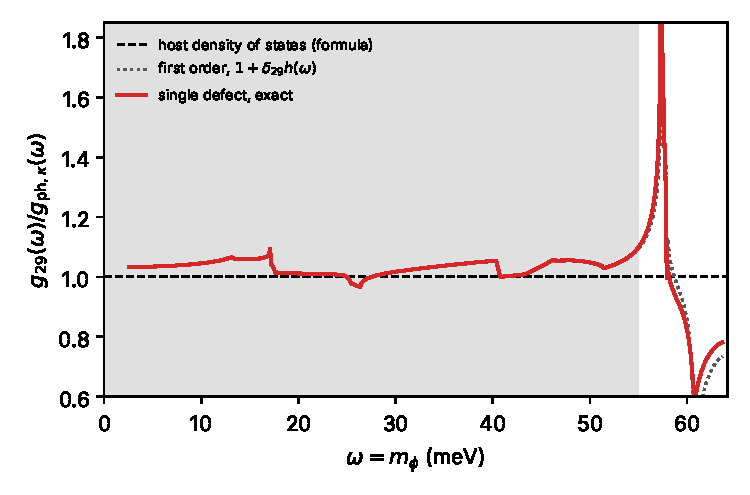
\includegraphics[width=\linewidth]{figures/ch11/limit11_6a.pdf}
\captionof{figure}{Rate of \cref{eq:11.6-alp} for natural silicon, where the spin sits on $^{29}$Si, with the exact local density of states of one $^{29}$Si atom from \cref{eq:11.6-lifshitz} (red), divided by the same rate with the host density of states (dashed, the formula), against the axion mass. The ratio $g_{29}/g_{\mathrm{ph},\kappa}$ does not depend on the couplings. Dotted: the first order in the mass defect, $1 + \delta_{29}h_{\mathrm{iso}}(\omega)$ with $\delta_{29} = -0.0317$, \cref{eq:11.6-first}. PBE density of states of \cref{sec:5.2}, $T = 0$. Gray: within \SI{10}{\percent} of the formula, $m_\phi < \SI{55.0}{meV} = 0.865\,\omega_{\mathrm{max}}$.}\label{fig:11-limit-6a}
\par}
\smallskip
Near the top of the optical band the heavier isotope moves weight from the band edge to just below it, and the host density of states errs by up to a factor of 2.
\end{limitbox}

Below \SI{55}{meV} the heavier spin carrier changes the rate by $-3.5$ to $+\SI{10}{\percent}$, mostly by 1 to \SI{5}{\percent} upward, and the first order of \cref{eq:11.6-first} reproduces the exact ratio to \SI{0.5}{\percent}. At the sharp lower edge of the optical band the ratio rises to about 2, with a peak of 2.05 at \SI{57.3}{meV} in the PBE spectrum, and between 60 and \SI{63}{meV} it falls to 0.6, with a minimum of 0.59 near \SI{60.7}{meV}. The band integral is unchanged, since both densities of states are normalized to three, so the weight is moved and not lost. This is the correlation between the vertex and the mass: the vertex sits on an atom whose mass, and therefore whose vibrations, differ from the average. Bloch and collaborators assume that the isotopes leave the phonon spectrum unchanged, which holds for the crystal as a whole when one isotope dominates~\cite[footnote~5]{bloch2025broadband}. The local spectrum at a minority isotope still differs, and in silicon the host density of states is good to \SI{10}{\percent} over \SI{86}{\percent} of the band.

\Cref{eq:11.6-lifshitz} itself treats one defect in a perfect host. How far does it carry into a crystal that contains many?

\begin{limitbox}[Lifshitz mass-defect Green function][lim:11.6b]
One atom of mass $\bar M(1 - \delta^M)$ in a harmonic host: $\GF_i = \GF_{\mathrm{h}}/(1 + \delta^M\bar M\omega^2\GF_{\mathrm{h}})$ on its site~\cites{lifshitz1956some}{dawber1963vibrations}.
\par\smallskip
{\centering
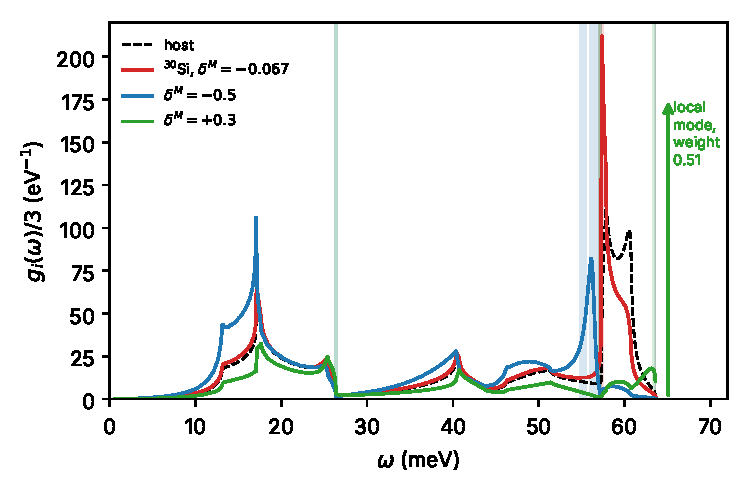
\includegraphics[width=\linewidth]{figures/ch11/limit11_6b.pdf}
\captionof{figure}{Local density of states per direction, $g_i(\omega)/3$, of one mass defect in silicon from \cref{eq:11.6-lifshitz}, with the PBE density of states of \cref{sec:5.2} (dashed, the host). Red: $^{30}$Si, $\delta^M = -0.067$. Blue: a heavy defect, $\delta^M = -0.5$. Green: a light defect, $\delta^M = +0.3$, which puts \SI{51}{\percent} of its weight into a local mode at \SI{65.1}{meV}, above the band (arrow). The integral of each curve, local mode included, is one. Shaded in the color of each curve: frequencies where the leading pair term exceeds \SI{10}{\percent}. The pair term is the effect of a second defect anywhere in the crystal on the first, for the natural isotope mixture around $^{30}$Si and for a concentration of \SI{1}{\percent} of the strong defects; pair term to first order in the scattering of the second defect, from the host Green function.}\label{fig:11-limit-6b}
\par}
\smallskip
The single-defect form fails where defects interact: within a meV of the sharp edges of the host density of states in natural silicon, and over windows of a few meV around them for defects of tens of percent in mass at concentrations of a percent.
\end{limitbox}

The pair term in the caption needs no new calculation. A second defect $j$ at site $\vect{r}$ changes the host function on site $I$ to $\GF_{\mathrm{h}} + \GF_{I\vect{r}}t_j\GF_{\vect{r}I}$, with $t_j = -\delta^M_j\bar M\omega^2/(1 + \delta^M_j\bar M\omega^2\GF_{\mathrm{h}})$ its scattering strength, and the sum over all $\vect{r} \neq I$ of $\GF_{I\vect{r}}\GF_{\vect{r}I}$ is $(\GF^2)_{II} - \GF_{\mathrm{h}}^2 = \partial\GF_{\mathrm{h}}/\partial(\bar M\omega^2) - \GF_{\mathrm{h}}^2$, since $\GF$ is the inverse of $\Phi - \bar M\omega^2$. For the natural mixture referenced to $\bar M$ the first order in the second defect cancels, $\sum_jx_j\delta^M_j = 0$, and what remains is of order $g_{\mathrm{md}} = \sum_jx_j(\delta^M_j)^2 = 2.0\times10^{-4}$, the mass variance of \cref{app:E.12}. It is the self-energy behind the isotope scattering of phonons: its imaginary part gives the width $\frac{\pi}{2}g_{\mathrm{md}}\,\omega^2g_{\mathrm{ph},\kappa}(\omega)/3$, which at low frequency is the Rayleigh rate of \cref{eq:E.12-iso}, and at \SI{50}{meV} is $2.5\times10^{-4}$ of $\omega$. For $^{30}$Si in natural silicon the pair term stays below \SI{2.2}{\percent} up to \SI{55}{meV} and passes \SI{10}{\percent} only within a meV of the sharp edge of the optical band at \SI{57}{meV}. In silicon the isotopes can be treated one at a time.

\subsection{Absorption of a baryon-minus-lepton vector}\label{sec:11.6-bl}

A vector boson can couple to baryon number minus lepton number, $B - L$, with strength $g_{B-L}$, the same for protons and neutrons, $+g_{B-L}$, and for electrons, $-g_{B-L}$ (\cref{sec:1.4}). A neutral atom of isotope $i$, with $A_i$ nucleons and $Z$ electrons, carries the charge $A_i - Z = N_i$, its neutron number. Light enough, the vector can be the dark matter, and it is then absorbed like a dark photon. At rest it couples to the spatial current of its charges (\cref{sec:8.1-absorption}),
\begin{equation*}
  g_{B-L}\Bigl[\sum_\kappa A_\kappa\vect{j}_\kappa - \vect{j}_e\Bigr] = g_{B-L}\sum_\kappa N_\kappa\vect{j}_\kappa + g_{B-L}\Bigl[\sum_\kappa Z_\kappa\vect{j}_\kappa - \vect{j}_e\Bigr] .
\end{equation*}
The bracket $\sum_\kappa Z_\kappa\vect{j}_\kappa - \vect{j}_e$ is the electric current in units of $e$, and that part of the coupling is a dark photon with $\zeta = g_{B-L}/e$, and its rate is the dark-photon rate with in-medium mixing, $\zeta^2\sigma_1/|\varepsilon|^2$ (\cref{sec:10.7}):
\begin{equation}
  \varGamma_{\mathrm{EM}} = \Bigl(\frac{g_{B-L}}{e}\Bigr)^2\omega\,\Imag\Bigl[-\frac{1}{\varepsilon(\omega)}\Bigr] ,
  \label{eq:11.6-GEM}
\end{equation}
at $\omega = m_\phi$, with $\sigma_1 = \omega\varepsilon_2$. In silicon this part creates no single phonon. Its one-phonon vertex is the Born charge, and the Born charges of silicon vanish (\cref{sec:5.5}). Below the electronic gap it is absorbed only by pairs of phonons, through the dipole that a displacement induces on top of another, which is the weak lattice absorption of silicon in the far infrared.

The neutron-number current $g_{B-L}\sum_\kappa N_\kappa\vect{j}_\kappa$ couples each nucleus to its neutron number. In a crystal of one isotope the vertex is $\ii\omega g_{B-L}N_\kappa\hat{\vect{\epsilon}}$, with $\hat{\vect{\epsilon}}$ the polarization of the vector. It is proportional to $M_\kappa$ on both sites of silicon, and the coupling-to-mass cancellation removes it: a monatomic crystal of one isotope does not absorb a $B - L$ vector into one phonon at all. Natural silicon does, because the neutron number per unit mass,
\begin{equation*}
  \mathfrak{b}_i = \frac{N_i}{M_i} ,
\end{equation*}
is $0.5004$, $0.5177$ and \SI{0.5338}{u^{-1}} for the three isotopes. The mass-proportional part of the vertex is set by the mass-weighted mean $\bar{\mathfrak{b}} = \sum_ix_iN_i/\sum_ix_iM_i = \SI{0.50235}{u^{-1}}$, with $x_i$ the abundances, and the remainder $\delta\vect{v}_I = \ii\omega g_{B-L}M_i(\mathfrak{b}_i - \bar{\mathfrak{b}})\hat{\vect{\epsilon}}$ has zero mean and is independent from site to site. Its direction is fixed, but on a cubic site every direction gives the same projection of the local density of states. \Cref{eq:11.6-random} with the vertex in $S_{OO}$ and \cref{eq:8.2-abs} give, per absorbed quantum at $T = 0$ and with $\Omega_{\mathrm{at}}$ the volume per atom,
\begin{keyresult}[Isotope-disorder absorption of a $B - L$ vector]
\begin{equation}
  \begin{aligned}
  \varGamma_{\mathrm{iso}}(\omega) &= \frac{\pi g_{B-L}^2}{2\Omega_{\mathrm{at}}}\sum_ix_iM_i(\mathfrak{b}_i - \bar{\mathfrak{b}})^2\,\frac{g_i(\omega)}{3} \\
  &= \frac{\pi g_{B-L}^2\bar M\sigma_{\mathfrak{b}}^2}{2\Omega_{\mathrm{at}}}\,\frac{g_{\mathrm{ph},\kappa}(\omega)}{3}\Bigl[1 + \langle\delta^M\rangle_{\mathfrak{b}}\,h_{\mathrm{iso}}(\omega) + O(g_{\mathrm{md}})\Bigr] ,
  \end{aligned}
  \label{eq:11.6-Giso}
\end{equation}
at $\omega = m_\phi$ inside the one-phonon band and zero above it, with $\sigma_{\mathfrak{b}}^2 = \sum_ix_i(M_i/\bar M)(\mathfrak{b}_i - \bar{\mathfrak{b}})^2$ the mass-weighted variance of $\mathfrak{b}$ and $\langle\delta^M\rangle_{\mathfrak{b}}$ the mass defect averaged with the weights $x_iM_i(\mathfrak{b}_i - \bar{\mathfrak{b}})^2$. In natural silicon $\sigma_{\mathfrak{b}}^2/\bar{\mathfrak{b}}^2 = 1.88\times10^{-4}$ and $\langle\delta^M\rangle_{\mathfrak{b}} = -0.054$.
\end{keyresult}
\noindent The two parts of the coupling reach different final states, one phonon or two, and they add without interference. The isotope phonons do not mix with the photon either, since the Born charge of every silicon atom vanishes whatever its mass. The vertex of an isotope sits on the atom whose mass differs. The isotope-resolved form of \cref{eq:11.6-Giso} takes this into account through the local density of states of each isotope, \cref{eq:11.6-lifshitz}, and the terms between different sites, which vanish to first order in the mass defects, are the pair terms of \cref{lim:11.6b}. A vector coupled to baryon number alone would see almost nothing. Its charge per mass, $A_i/M_i$, differs between the isotopes only through their binding energies, and the variance is $9\times10^{-11}$ of the squared mean, two million times below that of $B - L$.

How large is the isotope channel against the electromagnetic one? The answer depends on the temperature, through the two-phonon absorption. Consider a pair process in which the field is absorbed and two phonons of energies $\omega_1$ and $\omega_2$ are created, $\omega = \omega_1 + \omega_2$. Its rate is proportional to $(1 + n_1)(1 + n_2)$ and that of the reverse process, stimulated emission, to $n_1n_2$, with the Bose occupations $n_{1,2}$, so the net absorption carries $1 + n_1 + n_2 \ge 1$. In a difference process a phonon $\omega_2$ is absorbed and a phonon $\omega_1 = \omega + \omega_2$ created, with the net weight $n_2(1 + n_1) - n_1(1 + n_2) = n_2 - n_1 \ge 0$, which vanishes at $T = 0$. Suppose the second-order dipole moments and the phonon frequencies do not depend on temperature. Then every term of the absorption coefficient falls as the crystal cools, and
\begin{equation}
  \alpha(\omega; T \to 0) \le \alpha(\omega; \SI{293}{K}) .
  \label{eq:11.6-Tbound}
\end{equation}
The frequencies do shift, by about \SI{1}{\percent} between room temperature and zero, and the lines narrow, so the inequality holds for the absorption integrated over a window wider than the shift and the room-temperature width; where the room-temperature spectrum is flat over that window, it holds point by point. Below the top of the one-phonon band the far-infrared absorption of silicon at room temperature is dominated by difference processes~\cite{ikezawa1981far}, which freeze out completely, so the bound is far from saturated at millikelvin temperatures.

\begin{workedexample}{The isotope channel against the electromagnetic one at \SI{50}{meV}}\label{we:11-iso}
Take natural silicon and $m_\phi = \SI{50}{meV}$, inside the one-phonon band. With $\bar{\mathfrak{b}} = \SI{0.50235}{u^{-1}}$ and $\sigma_{\mathfrak{b}}^2 = 1.879\times10^{-4}\,\bar{\mathfrak{b}}^2 = \SI{4.742e-5}{u^{-2}}$, the product $\bar M\sigma_{\mathfrak{b}}^2 = \SI{1.332e-3}{u^{-1}}$ is \SI{1.430e-12}{eV^{-1}} with $\SI{1}{u} = \SI{931.494}{MeV}$. The PBE density of states of \cref{sec:5.2} gives $g_{\mathrm{ph},\kappa}/3 = \SI{15.9}{eV^{-1}}$ at \SI{50}{meV}, and the volume per atom is $\Omega_{\mathrm{at}} = a^3/8 = \SI{20.02}{\angstrom^3} = \SI{2.606e-9}{eV^{-3}}$. \Cref{eq:11.6-Giso} with the host density of states gives
\begin{equation*}
  \frac{\varGamma_{\mathrm{iso}}}{g_{B-L}^2} = \frac{\pi\times\SI{1.430e-12}{eV^{-1}}\times\SI{15.9}{eV^{-1}}}{2\times\SI{2.606e-9}{eV^{-3}}} = \SI{1.37e-2}{eV} .
\end{equation*}
The correction for the heavier carriers of the vertex is $\langle\delta^M\rangle_{\mathfrak{b}}h_{\mathrm{iso}} = (-0.054)(-1.55) = +\SI{8.3}{\percent}$ to first order, with $h_{\mathrm{iso}}(\SI{50}{meV}) = -1.55$ from the same density of states; the exact single-defect densities give $+\SI{8.0}{\percent}$, and $\varGamma_{\mathrm{iso}}/g_{B-L}^2 = \SI{1.48e-2}{eV}$.

For the electromagnetic part we need $\Imag(-1/\varepsilon)$ at \SI{50}{meV} (\SI{403}{cm^{-1}}). The measured absorption coefficient of silicon at \SI{293}{K} is $\alpha = \SI{0.55}{cm^{-1}}$ there~\cite{ikezawa1981far}; we read it off a published figure~\cite[Fig.~3]{deinzer2004two}, and the reading is uncertain by about \SI{10}{\percent}. With $\varepsilon_2 = \alpha n_r/\omega$, $n_r = 3.42$ and $\omega = \SI{2534}{cm^{-1}}$ as an inverse length ($2\pi$ times the wavenumber), $\varepsilon_2 = 7.43\times10^{-4}$, and with $\varepsilon_1 = 11.7$, $\Imag(-1/\varepsilon) = \varepsilon_2/(\varepsilon_1^2 + \varepsilon_2^2) = 5.42\times10^{-6}$. \Cref{eq:11.6-GEM} with $e^2 = 4\pi\alpha = 0.0917$ gives $\varGamma_{\mathrm{EM}}/g_{B-L}^2 = \SI{0.050}{eV}\times5.42\times10^{-6}/0.0917 = \SI{2.96e-6}{eV}$. By \cref{eq:11.6-Tbound} this is an upper bound at millikelvin temperatures, and
\begin{equation*}
  \frac{\varGamma_{\mathrm{iso}}}{\varGamma_{\mathrm{EM}}} \ge \frac{\SI{1.48e-2}{eV}}{\SI{2.96e-6}{eV}} = 5.0\times10^3 \qquad (\SI{50}{meV},\ T \to 0).
\end{equation*}
At \SI{50}{meV}, in a valley of the density of states between the longitudinal acoustic and optical features, the PBE spectrum, softer by about \SI{1}{\percent} than the room-temperature neutron data of \cref{sec:5.2}, shifts $g_{\mathrm{ph},\kappa}$ by a comparable amount. Neither this nor the reading of $\alpha$ changes the conclusion: in a cold silicon crystal a $B - L$ vector of \SI{50}{meV} is absorbed by the isotopes thousands of times more often than by the electromagnetic channel.
\end{workedexample}

\Cref{fig:11-iso} shows the two channels across the band. The isotope channel follows the density of states, from the acoustic peaks near \SI{17}{meV} to the optical peak near \SI{58}{meV}, and vanishes at the top of the band. Against the room-temperature electromagnetic bound it wins by factors from $2\times10^2$, at the top of the band where the density of states falls to zero, to $1.4\times10^4$. Above the band only the electromagnetic part remains, and at the two-phonon peak near \SI{76}{meV} it is 17 times stronger than at \SI{50}{meV}. The size of the isotope channel is set by the isotopic variance: a crystal enriched in $^{28}$Si suppresses it in proportion to the depletion of the minority isotopes, while the electromagnetic part is unchanged, which makes enrichment a control of the signal.

\begin{figure}[tbp]
  \centering
  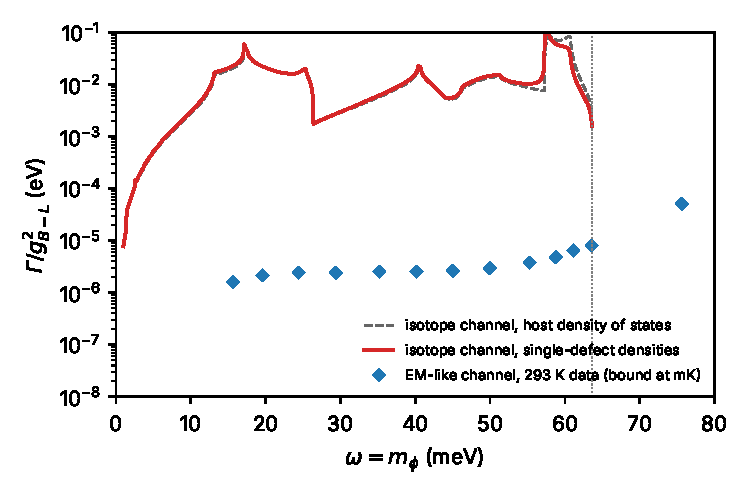
\includegraphics[width=0.8\linewidth]{figures/ch11/fig11_6.pdf}
  \caption{Absorption rate per quantum of a $B - L$ vector in natural silicon, over the squared coupling, against its mass. Red: the isotope-disorder channel of \cref{eq:11.6-Giso} with the exact single-defect densities of states of the three isotopes, \cref{eq:11.6-lifshitz}; dashed: the same with the host density of states for all. PBE phonons of \cref{sec:5.2}, $T = 0$; the dotted line marks the top of the PBE band, \SI{63.7}{meV} (the measured band top is \SI{64.1}{meV}). Blue diamonds: the electromagnetic channel \cref{eq:11.6-GEM}, from the measured absorption coefficient at \SI{293}{K} of Ikezawa and Ishigame~\cite{ikezawa1981far}, read from Fig.~3 of Deinzer and Strauch~\cite{deinzer2004two} with an uncertainty of about \SI{0.05}{cm^{-1}} plus \SI{10}{\percent}, converted with $n_r = 3.42$ and $\varepsilon_1 = 11.7$. At millikelvin temperatures the diamonds are upper bounds, \cref{eq:11.6-Tbound}. The diamond at \SI{76}{meV} is the two-phonon peak, above the one-phonon band.}
  \label{fig:11-iso}
\end{figure}

The inputs of these rates come from one harmonic calculation of the pure crystal. Its density of states and \cref{eq:11.6-lifshitz} give the local density of states of every isotope, and the force constants are those of \cref{sec:5.2} and \cref{app:E.4}. The exact rate of a disordered crystal includes every isotope and the pair terms. It comes from diagonalizing the Hessian of a supercell of a few thousand atoms with the isotopes drawn at random, and \cref{app:E.17} specifies that calculation; the single-defect correction of \cref{eq:11.6-Giso} is its check. The spin expectation values $\langle S_p\rangle$ and $\langle S_n\rangle$ of each odd isotope, which set $g_{ai}$ and $c_4^{(i)}$, come from nuclear shell-model calculations, and \cref{app:E.27} specifies them with their spread.

One input is missing. The electromagnetic channel of \cref{eq:11.6-GEM} needs $\varepsilon(\omega)$ of silicon inside the one-phonon band at the temperature of the detector, and we know of no measurement of the two-phonon absorption of silicon below \SI{65}{meV} at low temperature. The room-temperature data give only the bound \cref{eq:11.6-Tbound}, dominated by difference processes that are absent in a cold crystal. The zero-temperature absorption requires the second-order dipole moments, the derivatives of the Born charges with respect to the displacements, which a first-principles calculation can supply (\cref{app:E.17}); until it or a cold measurement exists, the margin of $5\times10^3$ at \SI{50}{meV} is a lower limit.
